\chapter{Décision de maintenance, économie et perspectives}

\chapintro
Une bonne prédiction ne sert que si elle aide à décider. Ce chapitre transforme les prédictions en stratégies de maintenance, compare leur coût, résume les indicateurs clés du projet et propose des pistes d'amélioration.

\section{Hypothèses de l'analyse économique}

Le jeu de données ne contient aucun coût : nous utilisons les hypothèses du tableau~\ref{tab:hypotheses}, exprimées en unités relatives (1 u = le coût d'un remplacement planifié, par exemple 1 000 DT). Elles sont modifiables en direct dans le tableau de bord, et l'étude de sensibilité ci-dessous montre leur effet.

\begin{table}[H]
\centering\small
\begin{tabularx}{\linewidth}{lcY}
\toprule
Paramètre & Valeur & Signification \\
\midrule
Coût d'un remplacement planifié $C_p$ & 1 u & pièce et main-d'œuvre, intervention prévue \\
Coût d'une panne $C_c$ & 5 u & intervention en urgence, arrêt de production, dégâts \\
Coût d'une fausse alarme & 0,1 u & une inspection pour rien \\
Délai d'intervention & 2 min & temps entre la décision et le remplacement (échelle de l'essai accéléré) \\
Seuil de décision $s$ & 10 min & on remplace quand la RUL prédite passe sous $s$ \\
\bottomrule
\end{tabularx}
\caption[Hypothèses de l'analyse économique]{Hypothèses de l'analyse économique.}
\label{tab:hypotheses}
\end{table}

\section{Optimisation de la maintenance préventive}

Avec la loi de Weibull, le coût par heure $C(T)$ d'un remplacement à l'âge $T$ est minimal pour $\boldsymbol{T^* = 224}$ \textbf{min} (figure~\ref{fig:economie}, à gauche) : on économise 23 \% par rapport au tout correctif, en théorie. Ce gain existe parce que $\beta > 1$ : un roulement vieux casse plus souvent qu'un neuf. Le tableau~\ref{tab:rapport} montre que l'âge optimal et le gain dépendent beaucoup du rapport $C_c/C_p$ : si une panne coûte à peine plus qu'un remplacement, le préventif ne sert à rien.

\begin{table}[H]
\centering\small
\begin{tabular}{lcccccc}
\toprule
Rapport $C_c / C_p$ & 1,5 & 2 & 3 & 5 & 7 & 10 \\
\midrule
Âge optimal $T^*$ (min) & 858 & 520 & 336 & 224 & 179 & 143 \\
Gain théorique / correctif & 0 \% & 2 \% & 10 \% & 23 \% & 32 \% & 41 \% \\
\bottomrule
\end{tabular}
\caption[Âge optimal selon le rapport des coûts]{Sensibilité de l'âge optimal au rapport des coûts.}
\label{tab:rapport}
\end{table}

\section{Comparaison des stratégies}

Nous rejouons maintenant la vraie vie des 11 roulements de test avec chaque stratégie (figure~\ref{fig:economie}, à droite, et tableau~\ref{tab:strategies-cout}).

\begin{figure}[H]
\centering
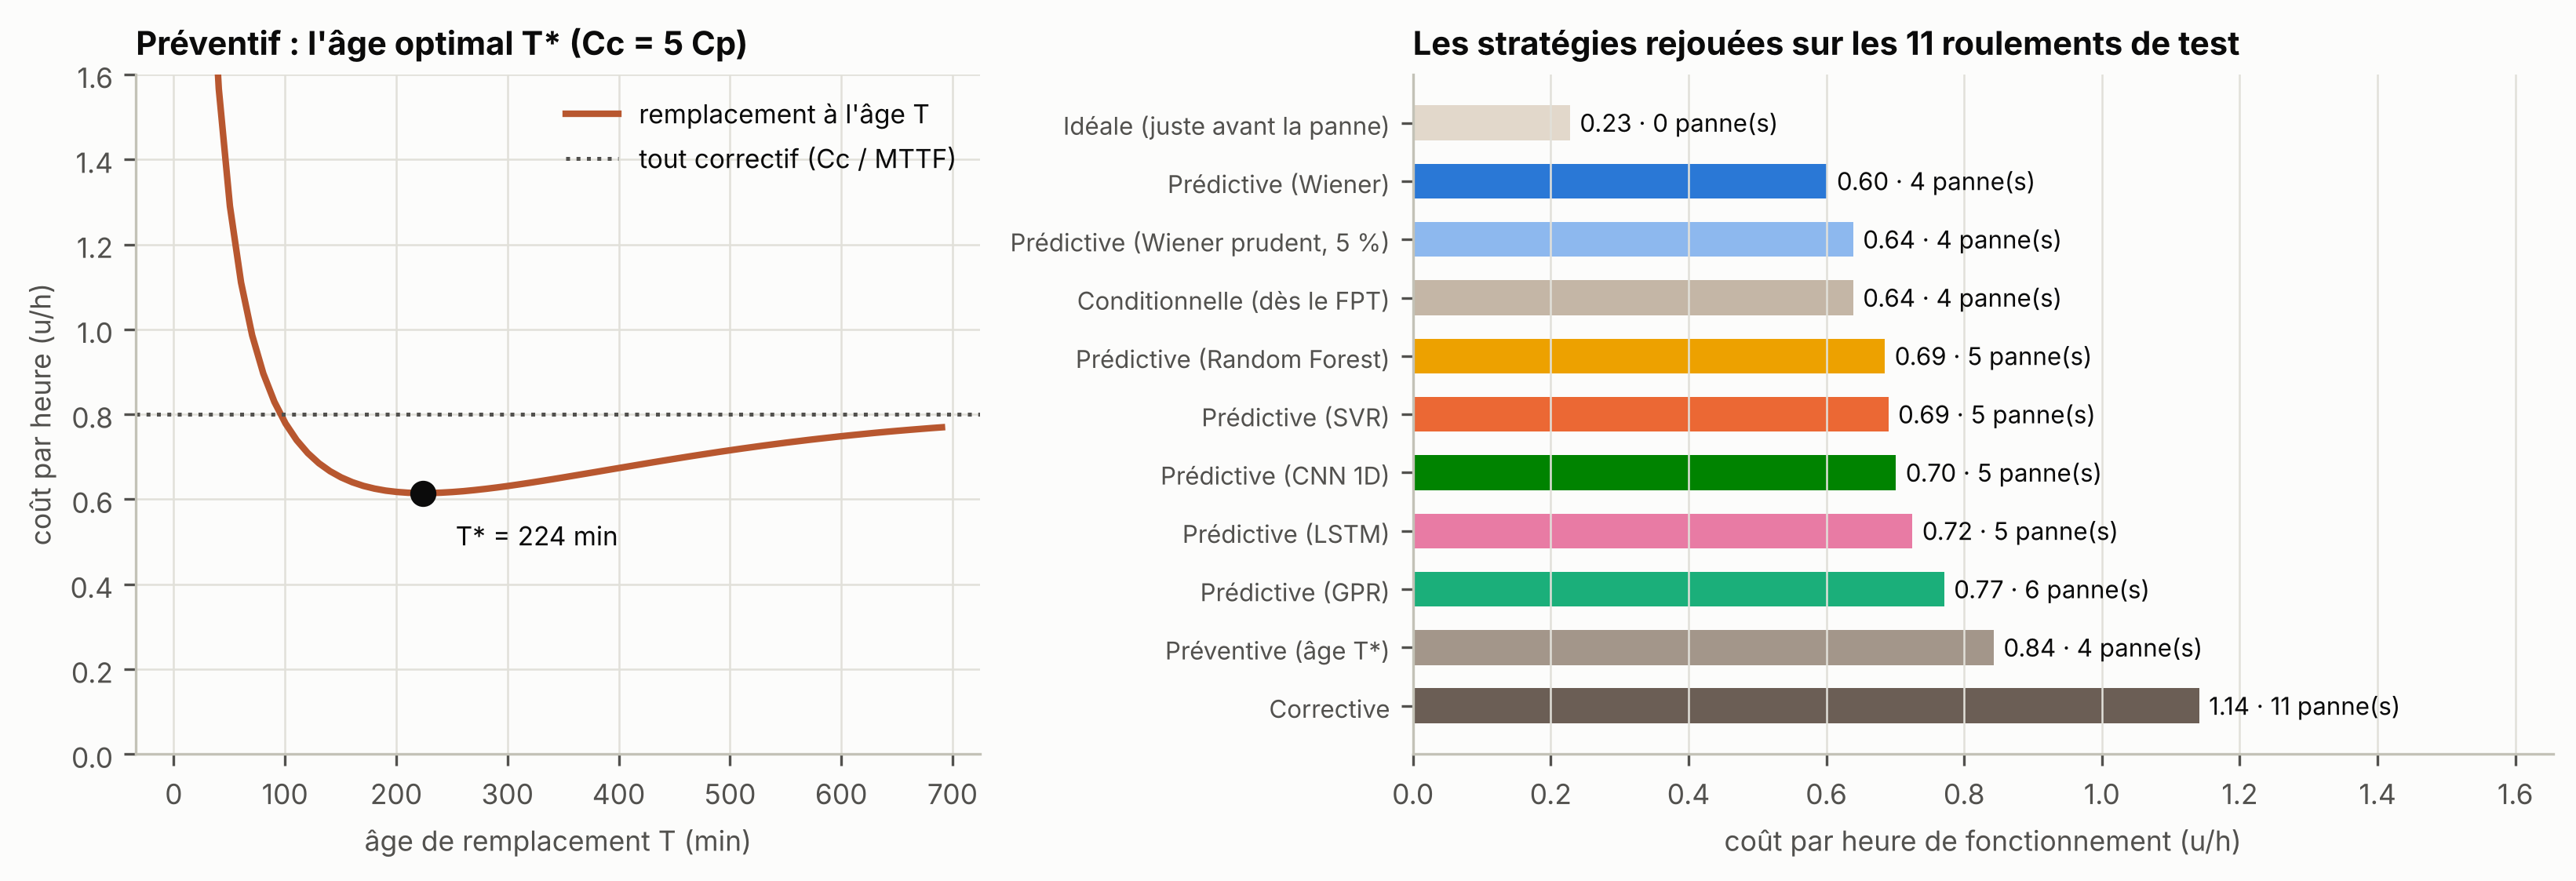
\includegraphics[width=\linewidth]{figures/fig22_economie.png}
\caption[Âge optimal et coût des stratégies]{À gauche : coût par heure d'un remplacement à l'âge $T$ et âge optimal $T^*$. À droite : coût par heure de chaque stratégie, rejouée sur les 11 roulements de test.}
\label{fig:economie}
\end{figure}

\begin{table}[H]
\centering\small
\begin{tabular}{lcccc}
\toprule
Stratégie & Coût (u/h) & Pannes (sur 11) & Vie gaspillée & Gain / correctif \\
\midrule
Corrective & 1,14 & 11 & 0 min & — \\
Préventive à l'âge $T^*$ & 0,84 & 4 & 139 min & 26 \% \\
Conditionnelle (dès le défaut) & 0,64 & 4 & 38 min & 44 \% \\
\textbf{Prédictive (Wiener)} & \textbf{0,60} & 4 & 14 min & \textbf{47 \%} \\
Prédictive (Wiener prudent, 5 \%) & 0,64 & 4 & 38 min & 44 \% \\
Prédictive (forêt aléatoire) & 0,68 & 5 & 15 min & 40 \% \\
Prédictive (SVR) & 0,69 & 5 & 18 min & 40 \% \\
Prédictive (CNN 1D) & 0,70 & 5 & 26 min & 39 \% \\
Prédictive (LSTM) & 0,73 & 5 & 41 min & 36 \% \\
Prédictive (GPR) & 0,77 & 6 & 18 min & 32 \% \\
Idéale (juste avant la panne) & 0,23 & 0 & 0 min & 80 \% \\
\bottomrule
\end{tabular}
\caption[Bilan économique des stratégies]{Bilan économique des stratégies sur les 11 roulements de test (vie gaspillée : moyenne sur les roulements remplacés avant la panne).}
\label{tab:strategies-cout}
\end{table}

Trois enseignements :
\begin{itemize}
  \item \textbf{Surveiller paie} : les stratégies conditionnelle et prédictives divisent presque le coût par deux par rapport au correctif, et font mieux que le préventif, qui jette en moyenne 139 min de vie par roulement.
  \item \textbf{La prédiction de la RUL apporte un gain de plus} : le Wiener utilise mieux la vie restante (14 min gaspillées au lieu de 38) sans ajouter de panne. C'est la meilleure stratégie réaliste (gain de 47 \%).
  \item \textbf{Les 4 pannes restantes sont inévitables avec des capteurs} : sur Bearing2\_3, Bearing2\_4, Bearing2\_6 et Bearing2\_7, le défaut apparaît 2 min ou moins avant la casse, ce qui ne laisse pas le temps d'intervenir. Le délai d'alerte doit être plus long que le délai d'intervention.
\end{itemize}
Le seuil $s$ se règle comme un hyperparamètre : trop petit, on intervient trop tard ; trop grand, on remplace dès l'alarme.

\section{Indicateurs clés (KPIs) du projet}

Le tableau~\ref{tab:kpis} rassemble les indicateurs clés, de la fiabilité jusqu'au coût.

\begin{table}[H]
\centering\small
\begin{tabularx}{\linewidth}{llY}
\toprule
Domaine & Indicateur & Valeur \\
\midrule
\multirow{3}{*}{Fiabilité} & MTTF & 375 min \\
& B10 / B50 & 125 min [78 ; 234] / 346 min [219 ; 573] \\
& Taux de défaillance à 300 min & 0,20 défaillance par heure \\
\midrule
\multirow{3}{*}{Détection} & Délai d'alerte médian (premier défaut → panne) & 7,8 min \\
& Fausses alarmes annulées & 14 (sur 8 roulements parmi 17) \\
& Tests dégradés à la troncature & 3 sur 11 \\
\midrule
\multirow{3}{*}{Pronostic} & Meilleure RMSE & 16,4 min (Wiener) \\
& Meilleur score PHM & 0,084 (LSTM) \\
& Couverture de l'intervalle à 90 \% & 54 \% (Wiener) \\
\midrule
\multirow{2}{*}{Économie} & Gain de la meilleure stratégie & $-47$ \% de coût par heure (Wiener prédictif) \\
& Pannes évitées & 7 sur 11 (64 \%) \\
\bottomrule
\end{tabularx}
\caption[Indicateurs clés de performance (KPIs)]{Indicateurs clés de performance du projet.}
\label{tab:kpis}
\end{table}

\section{Interprétation industrielle et limites}

En usine, la démarche s'utiliserait en deux temps : la fiabilité de la population fixe un plan de base (inspection, stock de pièces de rechange), puis la surveillance vibratoire déclenche l'intervention roulement par roulement. Nos résultats ont cependant des limites :
\begin{itemize}
  \item \textbf{peu de données} : 6 roulements d'apprentissage et des durées de vie de 38 à 467 min, même sous une même condition ;
  \item \textbf{défaillances brutales} : pour la plupart des roulements de test, le défaut détectable dure moins de 17 min ;
  \item \textbf{intervalles trop étroits} : l'intervalle du Wiener ne contient la vraie RUL que dans 54 \% des cas, à cause du seuil de défaillance ;
  \item \textbf{coûts et temps illustratifs} : l'essai est accéléré, et les coûts sont des hypothèses à remplacer par ceux de l'usine.
\end{itemize}

\section{Perspectives}

\begin{itemize}
  \item \textbf{Mieux modéliser la dégradation} : modèle exponentiel ou filtre particulaire, et un seuil de défaillance appris par condition opératoire.
  \item \textbf{Calibrer l'incertitude} : élargir les intervalles à partir des erreurs observées, par exemple avec la prédiction conforme, pour atteindre vraiment 90 \%.
  \item \textbf{Autres réseaux} : GRU et TCN, apprentissage par transfert d'une condition à l'autre \cite{dhungana2025}.
  \item \textbf{Plus de covariables} : température du roulement (mesurée sur certains essais PRONOSTIA), lubrification, profil de charge réel.
  \item \textbf{Explicabilité plus fine} : valeurs de Shapley pour expliquer chaque prédiction, pas seulement le modèle.
  \item \textbf{Déploiement} : calcul en temps réel près de la machine et alertes envoyées à l'équipe de maintenance.
\end{itemize}

\chapconclusion
La surveillance vibratoire, associée à une prédiction de la RUL, réduit le coût de maintenance d'environ moitié dans notre étude, à condition que le défaut soit détecté assez tôt pour intervenir. Le processus de Wiener offre le meilleur compromis entre précision, simplicité et explicabilité.
